%\documentclass[11pt,aspectratio=169]{beamer}
\documentclass[11pt,aspectratio=169,handout]{beamer}

\usetheme{Boadilla}
\usepackage[utf8]{inputenc}
\usepackage[T1]{fontenc}
\usepackage{lmodern}
\usepackage{lipsum}
\usetheme{default}
\usepackage{listings}
\lstset{language=[90]Fortran,
	basicstyle=\small\ttfamily,
	showtabs=false,
	tabsize=2,      
	keywordstyle=\color{red},
	commentstyle=\color{green},
	morecomment=[l]{!\ }% Comment only with space after !
}


\begin{document}
\author{Zejian Li \\(li.zejian@ictp.it)}
\title{Lecture 2-1: Numerical Integration}
\subtitle{(Adapted from slides by Gerald Fux)}
%\logo{}
%\institute{}
\date{21. Oct. 2024}
%\subject{}
%\setbeamercovered{transparent}
%\setbeamertemplate{navigation symbols}{}


% ----------------------------------------------------------------
\begin{frame}[plain]
	\maketitle
\end{frame}


% ----------------------------------------------------------------
\section{Introduction}

\begin{frame}
\frametitle{Numerical Integration - Introduction}
\textbf{Numerical integration is ...}
\begin{itemize}
 \item ... about calculating the numerical value of a definite Integral of some function $f(x)$, such as (in 1 dimension): 
$$ \int_a^b f(x) \, \mathrm{d}x. $$
\end{itemize}

\pause
\textbf{Numerical integration is not necessary if ...}
\begin{itemize}
	\item ... we know an elementary expression for the primitive $F(x) = \int f(x) \mathrm{d}x$.
	Then
	$$ \int_a^b f(x) \, \mathrm{d}x = F(b) - F(a). $$
	\pause
\end{itemize}
For example:
$$ \int_0^t x^2 \sin(x) \, \mathrm{d}x = -2 + (2 - t^2) \cos(t) + 2 t \sin(t).$$
\end{frame}


\begin{frame}
\frametitle{Numerical Integration - Introduction}
\textbf{We need numerical integration because ...}
\begin{itemize}
	\item ... for many functions $f(x)$ the primitive function $F(x)$ is either
	\begin{itemize}
		\item unknown, or
		\item not expressible as elementary functions, such as $\int e^{-x^2}\, \mathrm{d}x$.
	\end{itemize}
	\pause
	For example:
	$$ \int_{-\infty}^{1} e^{-x^2}\,\mathrm{d}x \simeq 1.63305$$
	\pause
	\item ... sometimes we don't even know an elementary expression for $f(x)$, but it is itself the result of some numerical computation.
	\pause
	For example:
	$$ f(t) = \int_{-\infty}^{t} e^{-x^2} \,\mathrm{d}t \quad \rightarrow \quad \int_0^2 f(t) \,\mathrm{d}t = ?? $$
\end{itemize}
\end{frame}

\begin{frame}
\frametitle{Numerical Integration Through the Riemann Sum}
\onslide<1->Consider the definition of integrals via the \textbf{Riemann sum}:
\onslide<3->{
\begin{equation*}
	\int_a^b f(x) \, \mathrm{d} x \equiv \lim_{N \rightarrow \infty}  \left[ \sum_{k=0}^{N-1} f(x_k) \cdot h \right] \quad \text{with} \quad
	\begin{cases}
		h \equiv \frac{b-a}{N} \\
		x_k \equiv a + k \cdot h \\
		k = 0, \ldots, N-1
	\end{cases}	
\end{equation*}}


\onslide<4->{This is an approximation for finite $N$, but improves for growing $N$ and is exact for $N \rightarrow \infty$ \\(if the function is ``well-behaved'', i.e. \textit{Riemann integrable}).}
\onslide<2->{\vspace{-0.2cm}
\begin{figure}
\centering
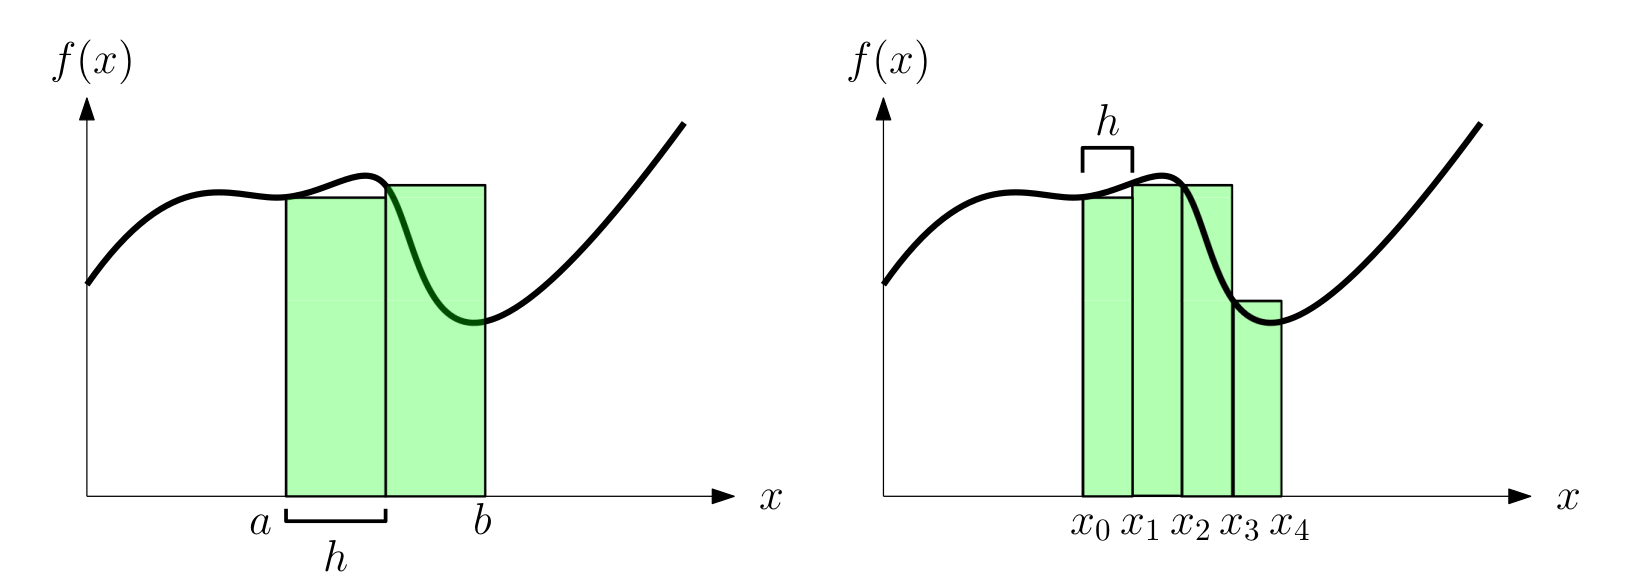
\includegraphics[width=0.75\textwidth]{fig/integration-definition}
\end{figure}
}
\end{frame}

\begin{frame}
\frametitle{Numerical Method: Left Riemann Sum}
\begin{columns}
\column{0.3\textwidth}
Define $I_L(N)$ as the approximated integral:
$$I_L(N) \equiv  \sum_{k=0}^{N-1} f(x_k) \cdot h$$ 
with
\begin{align*} 
	h & \equiv \frac{b-a}{N} \\
	x_k & \equiv a + k \cdot h \\
	k & = 0, \ldots, N-1.
\end{align*}

\pause

\column{0.65\textwidth}
\begin{block}{Algorithm: Left Riemann Sum}
\textbf{Input}: function $f(x)$; boundaries $a$ and $b$; small threshold $\epsilon$. \\
\pause
\begin{enumerate}
	\item Set $N$ to some initial value, e.g. $N:=32$
	\pause
	\item Compute $I_\mathrm{old} := I_L(N)$ 
	\pause
	\item Loop:
	\begin{itemize}
		\pause
		\item Increase $N$, e.g. $N := 2N$
		\pause
		\item Compute $I_\mathrm{new} := I_L(N)$
		\pause
		\item If $|I_\mathrm{new} - I_\mathrm{old}| < \epsilon$ then exit the loop, otherwise set $I_\mathrm{old} := I_\mathrm{new}$.
	\end{itemize}
\end{enumerate}
\pause
\textbf{Output}: $I_\mathrm{new}$, which is an approximate value of $\int_a^b f(x) \, \mathrm{d}x$
\end{block}
\end{columns}
\end{frame}

\begin{frame}
\frametitle{Numerical Method: Left Riemann Sum}
\begin{block}{Error scaling of the left Riemann sum}
For large enough $N$ the error decreases faster or as fast as $(1/N)^1$, i.e.
$$  \int_a^b f(x) \, \mathrm{d}x = I_L(N) + \mathcal{O}\left(\frac{1}{N}\right) $$
\end{block}
\end{frame}


\begin{frame}
	\frametitle{Improved Method (a): Midpoint Method}
	\begin{figure}
		\centering
		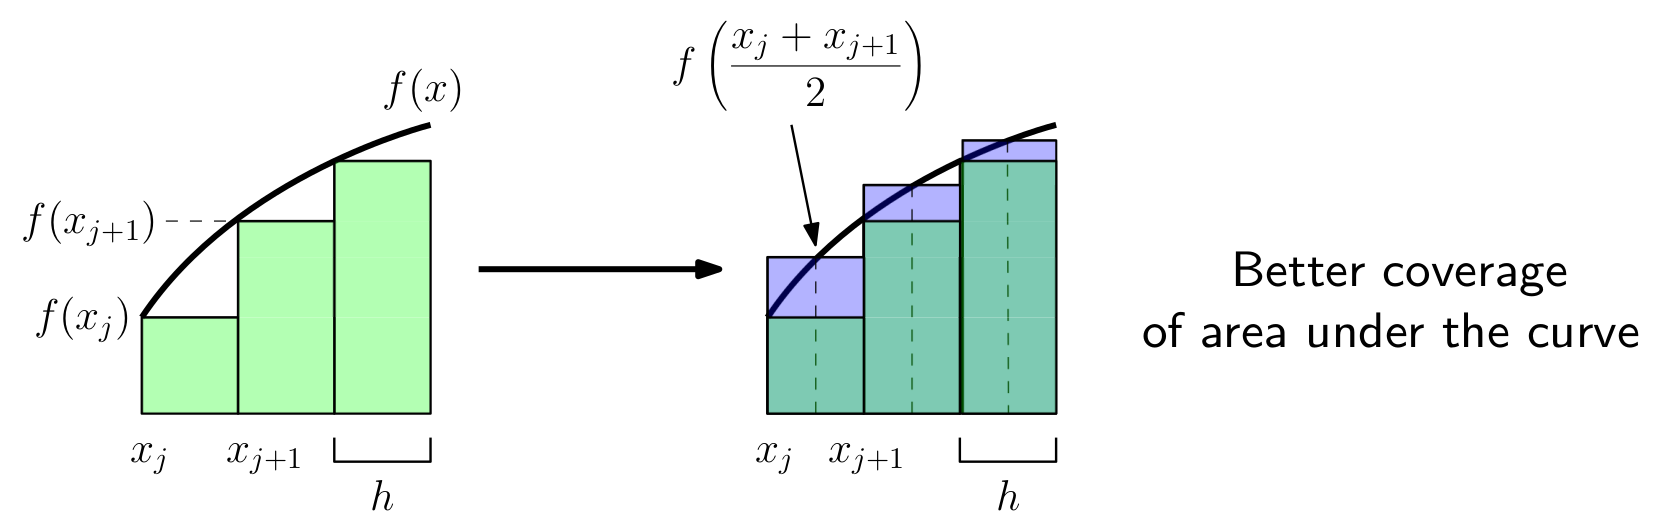
\includegraphics[width=0.8\textwidth]{fig/integration-midpoint-with-text}
	\end{figure}
	\pause
	\begin{equation*}
		I_M(N) \equiv  \sum_{k=0}^{N-1} f\left(\frac{x_k+x_{k+1}}{2}\right) \cdot h  \quad \text{with} \quad
		\begin{cases}
			h \equiv \frac{b-a}{N} \\
			x_k \equiv a + k \cdot h \\
			k = 0, \ldots, N-1
		\end{cases}
	\end{equation*}
	
	\only<3|handout:0>{
		Better convergence:
		\begin{equation*}
			\int_a^b f(x) \, \mathrm{d}x = I_M(N) + \mathcal{O}\left(\frac{1}{N^2}\right)
		\end{equation*}
	}
	
	\onslide<4>{
		Better convergence:
		\begin{equation*}
			\int_a^b f(x) \, \mathrm{d}x = I_M(N) + \mathcal{O}\left(\frac{1}{N^2}\right) =  I_M(h) + \mathcal{O}\left(h^2\right)
		\end{equation*}
	}
\end{frame}

\begin{frame}
	\frametitle{Improved Method (b): Trapezoidal Method}
	\begin{figure}
		\centering
		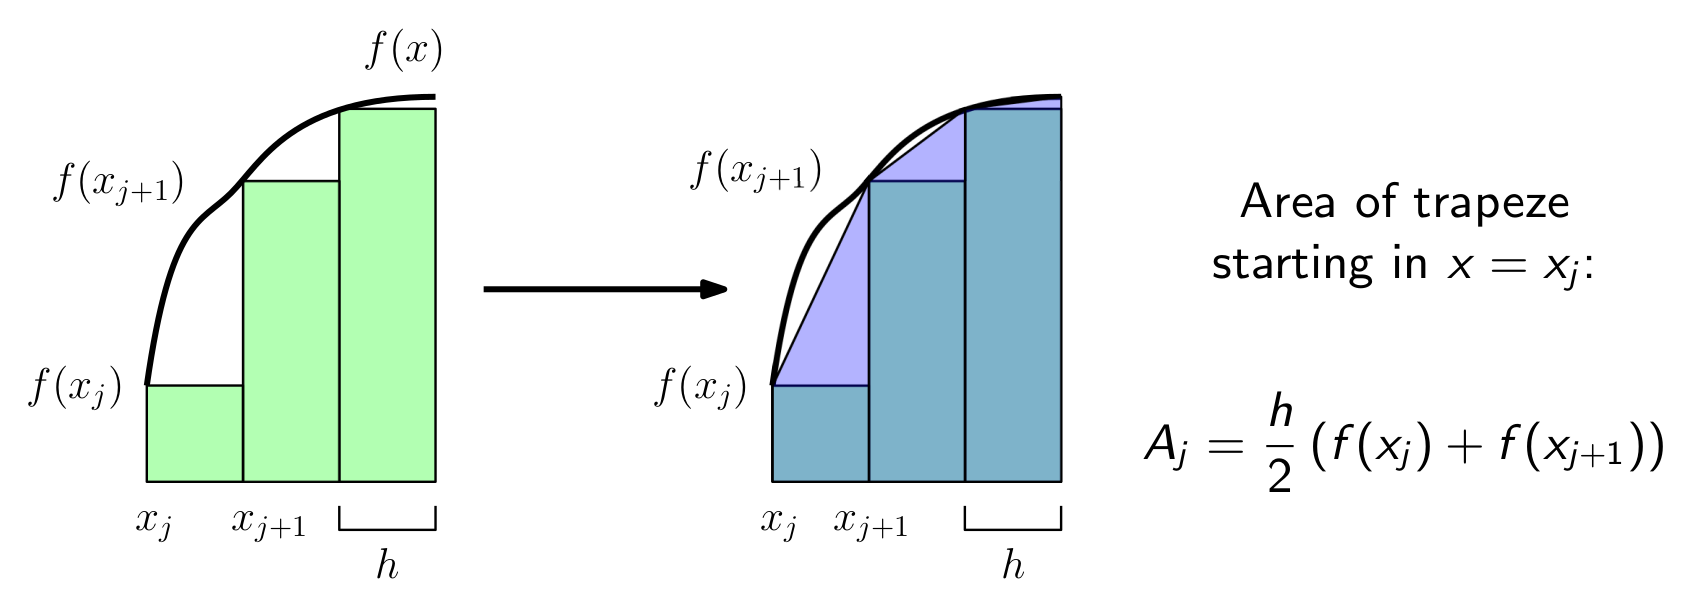
\includegraphics[width=0.7\textwidth]{fig/integration-trapez-with-text}
	\end{figure}
	\pause
	\begin{equation*}
		I_T(N) \equiv  \sum_{k=0}^{N-1} \left[ f(x_k)+f(x_{k+1}) \right] \cdot \frac{h}{2}  \quad \text{with} \quad
		\begin{cases}
			h \equiv \frac{b-a}{N} \\
			x_k \equiv a + k \cdot h \\
			k = 0, \ldots, N
		\end{cases}
	\end{equation*}
	
	\pause
	
	Convergence (same as the midpoint method):
	\begin{equation*}
		\int_a^b f(x) \, \mathrm{d}x = I_T(h) + \mathcal{O}\left(h^2\right)
	\end{equation*}
	
\end{frame}


\begin{frame}
	\frametitle{Improved Method (b): Trapezoidal Method}
	\begin{align*}
		I_T(N) & \equiv  \sum_{k=0}^{N-1} \left[ f(x_k)+f(x_{k+1}) \right] \cdot \frac{h}{2} \\
		& \equiv \frac{h}{2}\left[\underbrace{f(x_0) + f(x_1)} + \underbrace{f(x_1) + f(x_2)} + \underbrace{f(x_2) + f(x_3)} + \ldots \right]
	\end{align*}
	\begin{block}{(Better) reformulation of the trapezoidal method}
		Note that $f(x_1), f(x_2), \ldots, f(x_{N-2})$ each appear twice in the sum. Because it might be very hard to evaluate $f(x)$  it is better to \textbf{calculate each $f(x_j)$ only once instead of twice}. We thus implement the method in the rewritten form $\ldots$
		\begin{equation*}
			I_T(N) = \frac{h}{2} \left[ f(x_0) + \left(\sum_{k=1}^{N-1}  2f(x_k)\right)+f(x_{N}) \right] \mathrm{.}
		\end{equation*}
	\end{block}
	
\end{frame}

\begin{frame}
	\frametitle{Improved Method (c): Simpson Method}
	Next improvement: from Trapeziods $\rightarrow$ to \textbf{parabolic arcs.}
	\pause
	\begin{figure}
		\centering
		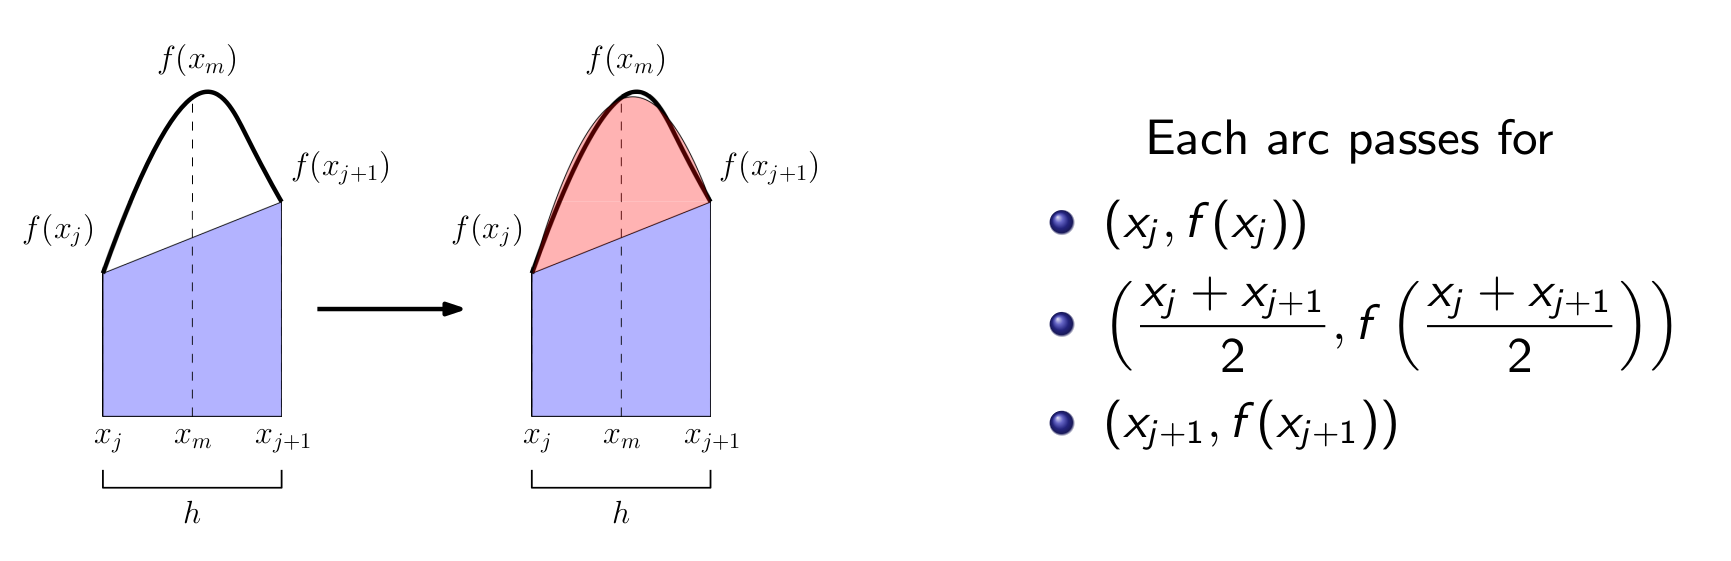
\includegraphics[width=0.7\textwidth]{fig/integration-simpson-with-text}
	\end{figure}%
	\pause
	\begin{equation*}
		\text{Algebra yields that the area is:} \quad A_j = \frac{h}{6} \left[ f(x_j) + 4 f\left(\frac{x_j + x_{j+1}}{2}\right) + f(x_{j+1}) \right]
	\end{equation*}
	
	\pause
	\begin{equation*}
		I_S(N) \equiv \frac{h}{6} \left[ f(x_0) + 2\sum_{k=1}^{N-1} f(x_k)+4\sum_{k=0}^{N-1}f\left(\frac{x_k + x_{k+1}}{2}\right) + f(x_{N}) \right] 
		\quad \text{with} \quad
		\begin{cases}
			h \equiv \frac{b-a}{N} \\
			x_k \equiv a + k \cdot h \\
			k = 0, \ldots, N
		\end{cases}
	\end{equation*}
	
\end{frame}

\begin{frame}
	\frametitle{Improved Method (c): Simpson Method}
	\begin{figure}
		\centering
		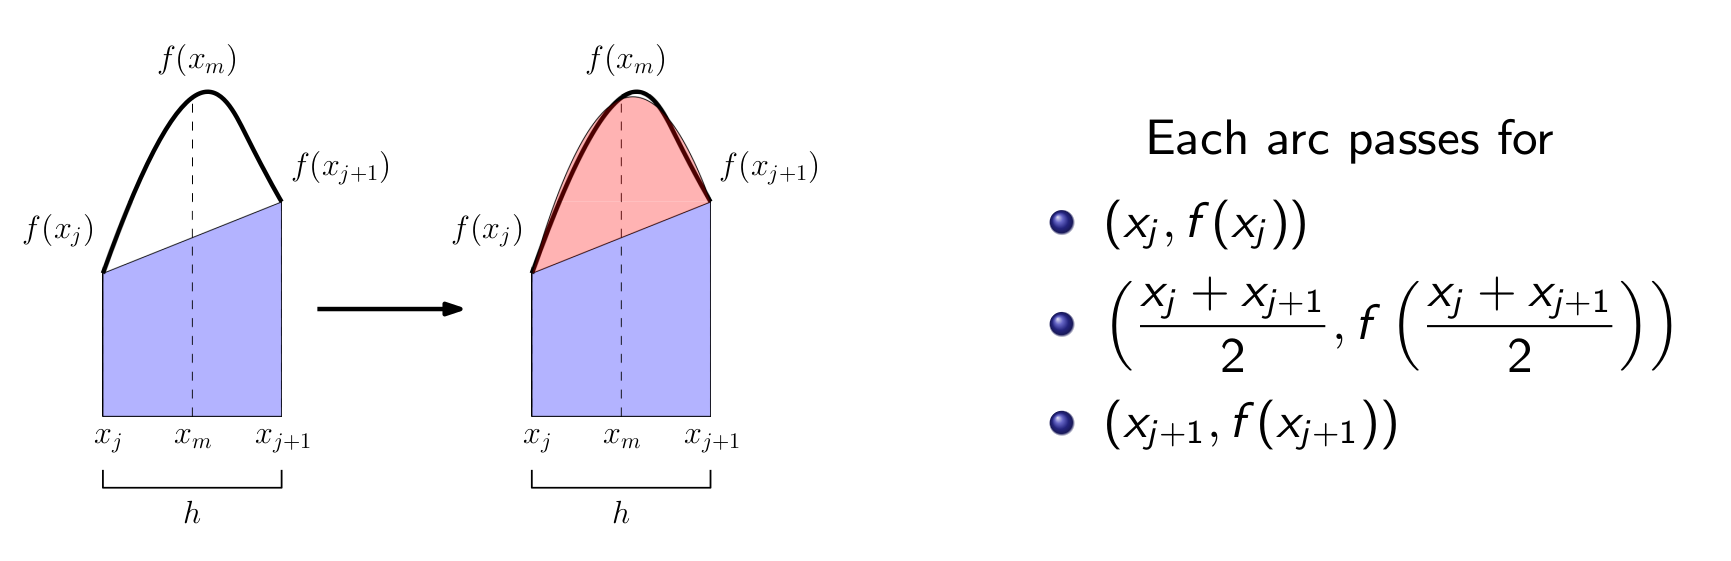
\includegraphics[width=0.7\textwidth]{fig/integration-simpson-with-text}
	\end{figure}%
	\begin{equation*}
		I_S(N) \equiv \frac{h}{6} \left[ f(x_0) + 2\sum_{k=1}^{N-1} f(x_k)+4\sum_{k=0}^{N-1}f\left(\frac{x_k + x_{k+1}}{2}\right) + f(x_{N}) \right] 
		\quad \text{with} \quad
		\begin{cases}
			h \equiv \frac{b-a}{N} \\
			x_k \equiv a + k \cdot h \\
			k = 0, \ldots, N
		\end{cases}
	\end{equation*}
	
	Convergence:
	\begin{equation*}
		\int_a^b f(x) \, \mathrm{d}x = I_S(h) + \mathcal{O}\left(h^4\right)
	\end{equation*}
	
\end{frame}

\begin{frame}
	\frametitle{Advanced Integration Methods}
	Beyond these basic approaches many advanced / specialized methods exist. E.g.:
	\pause
	\begin{columns}
		\column{0.6\textwidth}
		\textbf{Adaptive integration}: \\
		Make the grid finer where the function changes faster.
		\column{0.4\textwidth}
		\begin{figure}
			\centering
			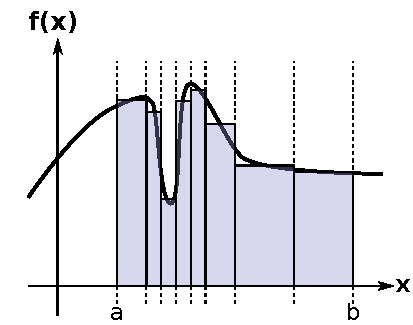
\includegraphics[width=0.4\textwidth]{fig/integration-adaptive}
		\end{figure}%
	\end{columns}
	
	\pause
	\begin{columns}
		\column{0.6\textwidth}
		\textbf{Gaussian quadratures}: \\
		Mathematically optimal grid.
		\column{0.4\textwidth}
		\begin{figure}
			\centering
			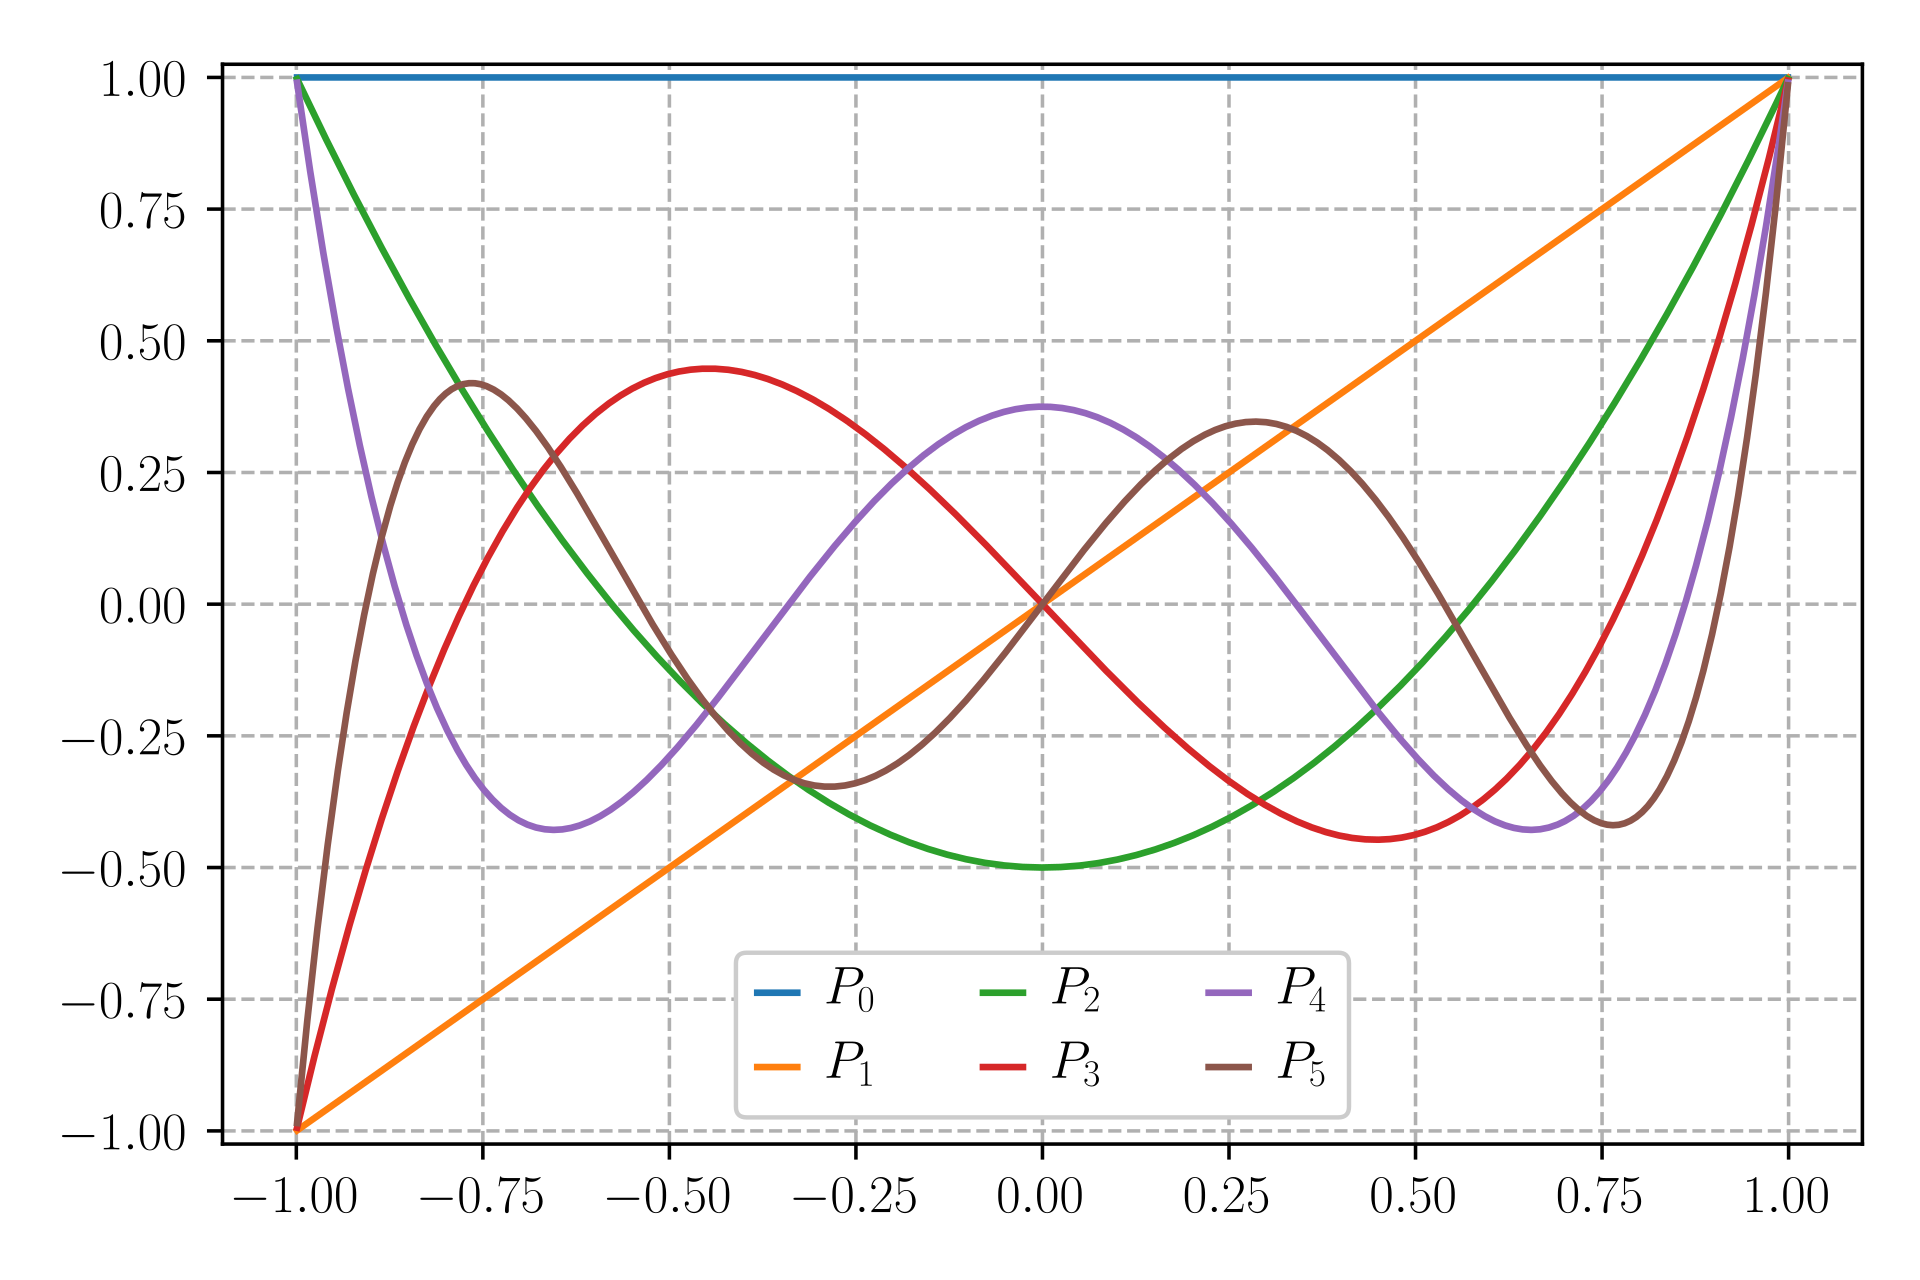
\includegraphics[width=0.4\textwidth]{fig/integration-legendre}
		\end{figure}%
	\end{columns}
	
	\pause
	\begin{columns}
		\column{0.6\textwidth}
		\textbf{Monte Carlo integration}: \\
		Use a randomized grid; best in high dimensions.
		\column{0.4\textwidth}
		\begin{figure}
			\centering
			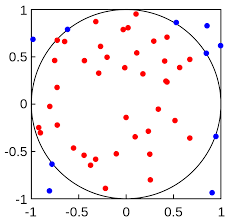
\includegraphics[width=0.3\textwidth]{fig/integration-monte-carlo}
		\end{figure}%
	\end{columns}
	
\end{frame}


\begin{frame}
\frametitle{Assignment 9}
Write a FORTRAN program that computes $\int_a^b f(x)\, \mathrm{d}x$ for  $f(x) = \dfrac{16x-16}{x^4 - 2x^3+4x-4}$.% using the left Riemann sum method:
\begin{itemize}
\item Write a function that takes the bounds $a$ and $b$, and the desired precision $\epsilon$.
\pause
\item The function should integrate with the left Riemann sum, increasing N until the precision is achieved.
\pause
\item The function should print the result at each step together with the current value for $N$ (this is just for us to see what is happening).
\pause
\item Test the function by calculating $\int_0^1 f(x)\, \mathrm{d}x$ with error threshold $\epsilon=10^{-5}$ in the main program and print the result. (Can you recognize the result?)
\pause
\item Submit your code as \texttt{Ass11.YourLastName.f90} to \texttt{li.zejian@ictp.it} before the next lesson.
\end{itemize}
\textbf{Hints:}
\begin{itemize}
\item Create separate functions for $f(x)$, the Riemann sum and the integration.
\end{itemize}
\pause
\textbf{Bonus question:}
\begin{itemize}
	\item Implement one (or as as many as you like) of the improved methods and compare their performance.
%	\item What happens if we don't increase $N$ significantly in each iteration (e.g. $N:=N+1$) ?  Can we trust the ``precision'' $\epsilon$? 
\end{itemize}

\end{frame}

\end{document}